\chapter{Metodología propuesta}\label{chapter:proposal}
\section{Asimetría}

\section{Simulación de la asimetría multivariante}

\begin{equation}
    A \cdot (1-e^{-S \cdot B})
\end{equation}

\begin{figure}[htbp]
    \centering
    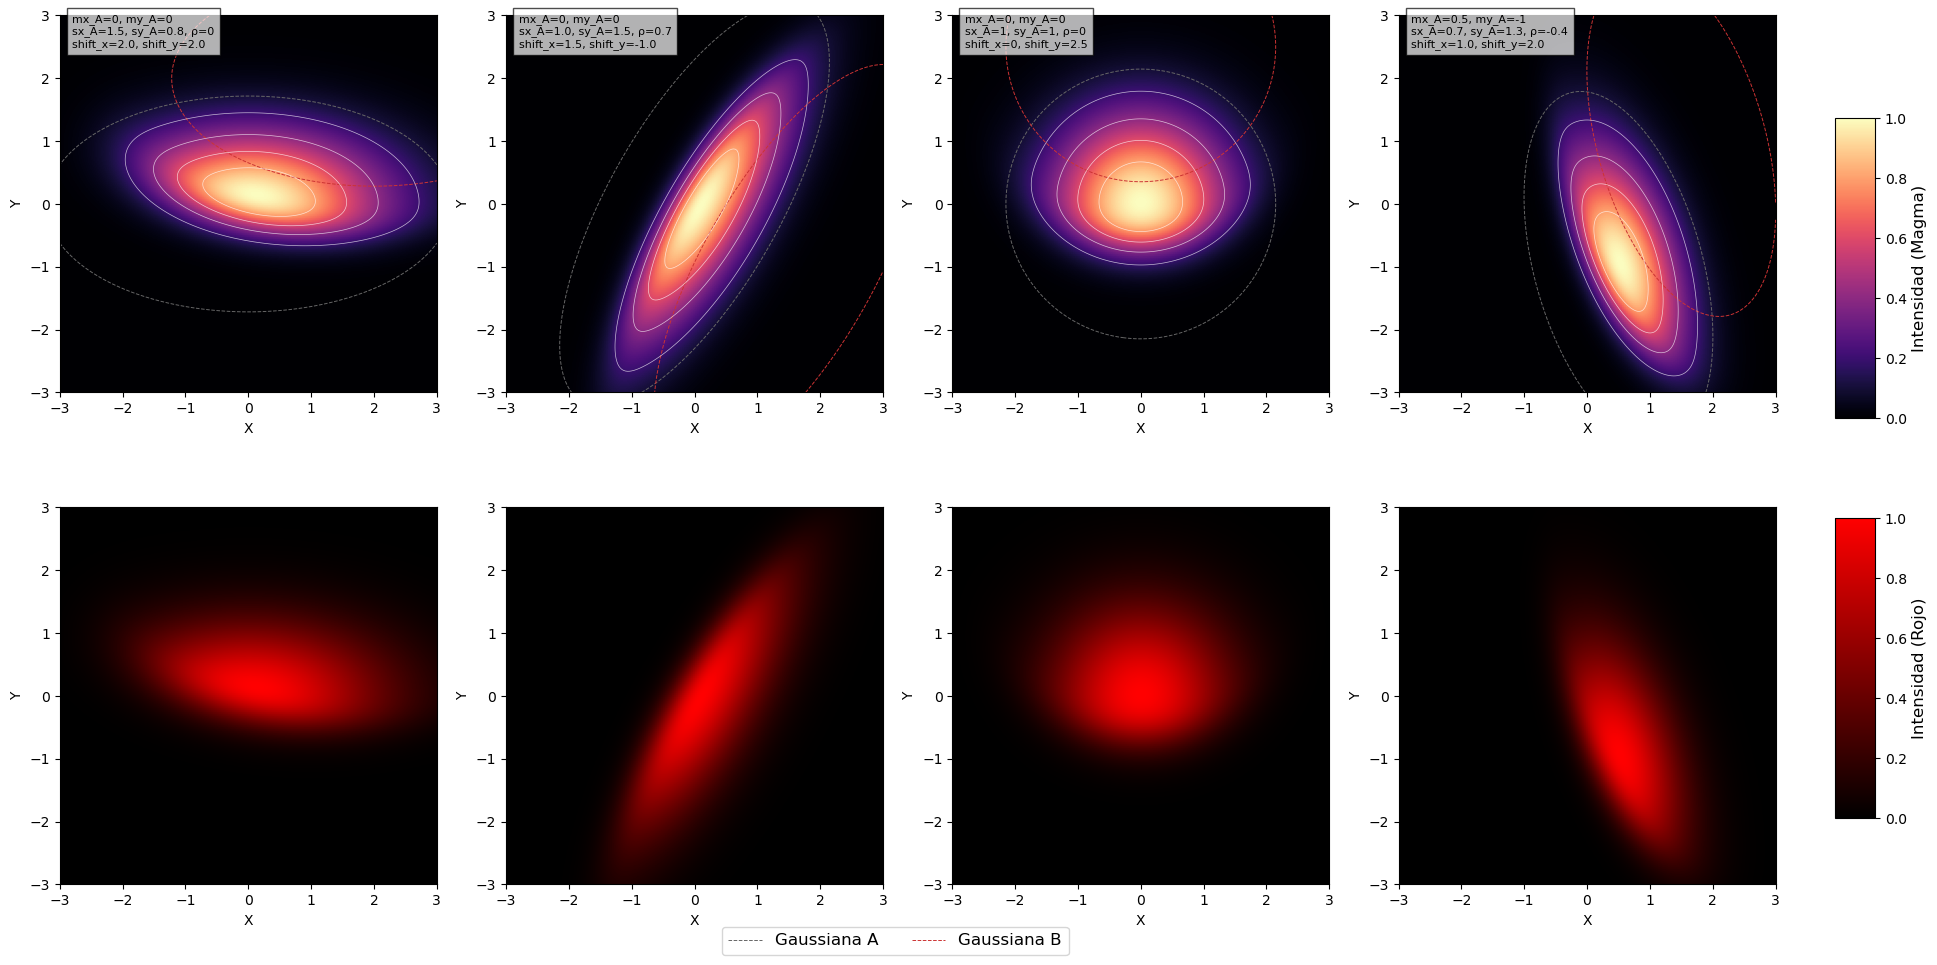
\includegraphics[width=1\textwidth]{Graphics/splatts.png}
    \caption{Visualización de la función de combinación \(A \cdot (1 - e^{-S B})\), utilizada para simular la asimetría. 
    Se muestran cuatro configuraciones distintas de parámetros. 
    La fila superior incluye mapas de calor con contornos de las gaussianas originales \(A\) y \(B\), 
    mientras que la fila inferior muestra únicamente la distribución combinada en escala monocroma sobre fondo negro.}
    \label{fig:gaussianas_2d_skewness}
\end{figure}

    
\section{Propagación de gradientes analítica}


\paragraph{Definición de la función de máscara.}

La opacidad de un píxel modificada por el skewness se define como:

\begin{equation}
M = A \left(1 - e^{-S B} \right)
\end{equation}

donde:
\begin{itemize}
    \item \( A = \alpha e^{-Q(d)} \) es la Gaussiana centrada en el punto original,
    \item \( B = \alpha e^{-Q(d - \vec{s})} \) es la Gaussiana desplazada por \( \vec{s} \),
    \item \( d \) es la diferencia entre la posición del píxel y el centro de la Gaussiana,
    \item \( \vec{s} \) es el desplazamiento en 2D causado por el skew,
    \item \( S \) es la sensibilidad del skew,
    \item \( Q(u) = \frac{1}{2} u^\top \Sigma^{-1} u \) es la forma cuadrática asociada a la inversa de la matriz de covarianza.
\end{itemize}

\paragraph{Derivada de \( M \) respecto al centro \( \vec{\mu} \).}

\begin{equation}
\frac{\partial M}{\partial \vec{\mu}} = -A \, \Sigma^{-1} d \, (1 - e^{-S B}) + A \, S \, e^{-S B} \, B \, \Sigma^{-1}(d - \vec{s})
\end{equation}

\paragraph{Derivada de \( M \) respecto al skew \( \vec{s} \).}

\begin{equation}
\frac{\partial M}{\partial \vec{s}} = A \, S \, e^{-S B} \, B \, \Sigma^{-1}(d - \vec{s})
\end{equation}

\paragraph{Derivada de \( M \) respecto a la sensibilidad del skew \( S \).}

\begin{equation}
\frac{\partial M}{\partial S} = A \, B \, e^{-S B}
\end{equation}

\paragraph{Relación entre el skew en 3D y el desplazamiento en 2D.}

El desplazamiento en pantalla debido al skew tridimensional está dado por:

\begin{equation}
\vec{s}_{2D} = \Pi(\vec{\mu}_{3D} + \vec{skew}_{cam}) - \Pi(\vec{\mu}_{3D})
\end{equation}

El gradiente de \( M \) respecto al skew en 3D es:

\begin{equation}
\frac{\partial M}{\partial \vec{skew}_{3D}} = R_{\text{cam}}^\top \cdot J_{\Pi}^\top \cdot \frac{\partial M}{\partial \vec{s}_{2D}}
\end{equation}

donde:
\begin{itemize}
    \item \( R_{\text{cam}} \) es la matriz de rotación del sistema global al sistema de la cámara,
    \item \( J_{\Pi} \) es el Jacobiano de la transformación de proyección.
\end{itemize}


\section{Complejidad computacional y análisis de estabilidad numérica}
\section{Ventajas teóricas sobre GS clásico}
